\documentclass[12pt,a4paper,twoside,openright,titlepage,final]{article}
\usepackage{fontspec}
\usepackage{amsmath}
\usepackage{amsfonts}
\usepackage{amssymb}
\usepackage{makeidx}
\usepackage{graphicx}
\usepackage[hidelinks,unicode=true]{hyperref}
\usepackage[spanish,es-nodecimaldot,es-lcroman,es-tabla,es-noshorthands]{babel}
\usepackage[left=3cm,right=2cm, bottom=4cm]{geometry}
\usepackage{natbib}
\usepackage{microtype}
\usepackage{ifdraft}
\usepackage{verbatim}
\usepackage[obeyDraft]{todonotes}
\ifdraft{
	\usepackage{draftwatermark}
	\SetWatermarkText{BORRADOR}
	\SetWatermarkScale{0.7}
	\SetWatermarkColor{red}
}{}
\usepackage{booktabs}
\usepackage{longtable}
\usepackage{calc}
\usepackage{array}
\usepackage{caption}
\usepackage{subfigure}
\usepackage{footnote}
\usepackage{url}
\usepackage{tikz}
\usepackage{pdflscape}
\usepackage{minted}

\setsansfont[Ligatures=TeX]{texgyreadventor}
\setmainfont[Ligatures=TeX]{texgyrepagella}

%*******************************************************
%                 NO MODIFICAR
\newcommand*{\FSfont}[1]{%
  \fontencoding{T1}\fontfamily{#1}\selectfont}

\newlength{\tpheight}\setlength{\tpheight}{0.9\textheight}
\newlength{\txtheight}\setlength{\txtheight}{0.9\tpheight}
\newlength{\tpwidth}\setlength{\tpwidth}{0.9\textwidth}
\newlength{\txtwidth}\setlength{\txtwidth}{0.9\tpwidth}
\newlength{\drop}
%*******************************************************

% Crea una portada con los siguientes parámetros
%
% #1 : Título 
% #2 : Subtítulo
% #3 : Subsubtítulo
% #4 : Autor(es)
% #5 : Lugar
%

\newcommand*{\portada}[5]{
\begin{titlepage}
\begingroup
\vspace*{1cm}
\drop = 0.2\txtheight
\centering
\vfill
{\Huge \scshape #1}\\[\baselineskip]
{\Large \textbf{#2}}\\[\baselineskip]
{\Large \scshape #3}\\[\baselineskip]
\vspace*{0.3cm}
{\large \textit{#4}}\\[0.5\drop]

\includegraphics[scale=0.35]{./imagenes/logoURJC.jpg}
\vspace*{1.5cm}

{\large \scshape #5, \today} \par
\begin{center}
\end{center}
\vfill\null
\endgroup
\end{titlepage}
}
 %*****************************************************
 


\author{José Ignacio Escribano}

\title{Caso práctico II: Generación de variables aleatorias}

\setlength{\parindent}{0pt}

\begin{document}

\pagenumbering{alph}
\setcounter{page}{1}

\portada{Caso práctico II}{Simulación y Metaheurísticas}{Generación de variables aleatorias}{José Ignacio Escribano}{Móstoles}

\listoftables
\thispagestyle{empty}
\newpage

\tableofcontents
\thispagestyle{empty}
\newpage


\pagenumbering{arabic}
\setcounter{page}{1}

\section{Introducción}

En este caso práctico utilizaremos distintos métodos para generar variables aleatorias; tanto unidimensionales como multidimensionales. En el primer caso generaremos la distribución exponencial y la normal. En el caso multidimensional, generaremos la normal.

\section{Resolución del caso práctico}

A continuación resolveremos cada una de las cuestiones planteadas.

\subsection{Cuestión 1}

Usando el comando \texttt{rnorm} generaremos 10, 100 y 10000 observaciones de una distribución normal de parámetros ($\mu = 3, \sigma^2 = 6^2$).\\

La Figura~\ref{fig:Rplot} muestra los histogramas con cada número de muestras.\\

\begin{figure}[htbp!]
\centering
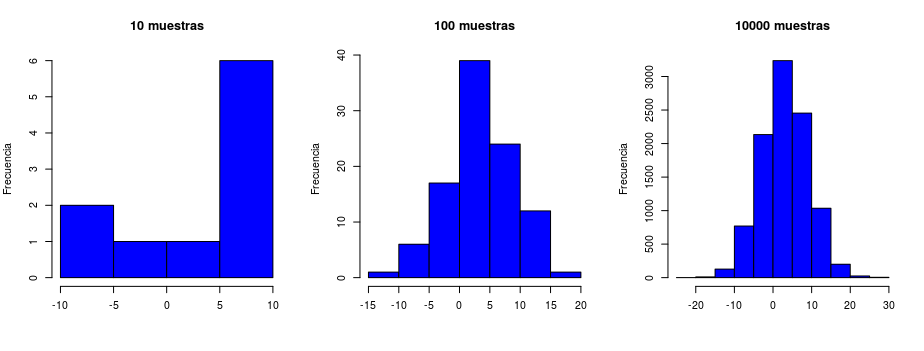
\includegraphics[width=0.8\linewidth]{imagenes/Rplot}
\caption{Histograma de una distribución normal con 10, 100 y 10000 muestras}
\label{fig:Rplot}
\end{figure}

Se puede observar como, a medida que se aumenta el número de muestras de la distribución, el histograma toma la forma característica de una distribución normal: simétrica y con forma de campana.\\

Usaremos distintos estadísticos muestrales para comprobar el hecho anterior. Estos estadísticos serán la media, varianza, primer y tercer cuartil, la desviación típica, la moda, el kurtosis y la asimetría. \\

La Tabla~\ref{tbl:comp} muestra una comparativa de los distintos estadísticos según el número de muestras de la distribución normal.\\

\begin{table}[htbp!]
\centering
\caption{Comparativa de distintos parámetros muestrales de tres distribuciones normales con distinto número de muestras}
\label{tbl:comp}
\resizebox{\textwidth}{!}{%
\begin{tabular}{@{}cccccccccc@{}}
\toprule
\textbf{Distribución}                                                                                & \textbf{Media} & \textbf{Varianza} & \textbf{1Q} & \textbf{3Q} & \textbf{\begin{tabular}[c]{@{}c@{}}Desviación\\ típica\end{tabular}} & \textbf{Moda} & \textbf{Kurtosis} & \textbf{Asimetría} & \textbf{Mediana} \\ \midrule
\begin{tabular}[c]{@{}c@{}}$\mathcal{N}(\mu = 3, \sigma^2 = 6 ^2)$\\ con 10 muestras\end{tabular}    & 2.788          & 35.593            & -2.168      & 6.826       & 5.966                                                                & 2.788         & 1.820             & -0.767             & 5.735            \\ \hline
\begin{tabular}[c]{@{}c@{}}$\mathcal{N}(\mu = 3, \sigma^2 = 6 ^2)$\\ con 100 muestras\end{tabular}   & 3.537          & 31.452            & 0.148       & 7.501       & 5.608                                                                & 3.537         & 3.319             & -0.129             & 3.573            \\ \hline
\begin{tabular}[c]{@{}c@{}}$\mathcal{N}(\mu = 3, \sigma^2 = 6 ^2)$\\ con 10000 muestras\end{tabular} & 3.089          & 36.470            & -0.954      & 6.039       & 7.172                                                                & 3.088         & 3.045             & 0.021              & 3.0340           \\ \hline
$\mathcal{N}(\mu = 3, \sigma^2 = 6 ^2)$                                                              & 3              & 36                & -1.046      & 7.046       & 6                                                                    & 3             & 3                 & 0                  & 3                \\ \bottomrule
\end{tabular}%
}
\end{table}

Se puede observar que, según aumentamos el número de muestras que tomamos, los resultados de los estadísticos se acercan más a los resultados analíticos. Hay que tener en cuenta que para tener un resultado más fiable habría que repetir la simulación varias veces y calcular la media de esas simulaciones.


\subsection{Cuestión 2}

\subsection{Cuestión 3}

\subsection{Cuestión 4}

\section{Conclusiones}


\newpage

\section{Código R utilizado}

A continuación se muestra el código utilizado para la realización de este caso práctico.


\end{document}